%set the master document for easy compilation
%!TEX root = ../D3_5_3.tex

\section{F2.7: SpeedSupervision\_Integration}

\subsection{Component Requirements}

\begin{longtable}{p{.25\textwidth}p{.7\textwidth}}
\toprule
Component name			& SpeedSupervision\_Integration\\
\midrule
Link to SCADE model		& {\footnotesize \url{https://github.com/openETCS/modeling/tree/master/model/Scade/System/ObuFunctions/SpeedSupervison}} \\
\midrule
SCADE designer			& Benjamin Beichler, University of Rostock\newline
Christian Stahl, TWT\newline
Thorsten Schulz, University of Rostock \\
\midrule
Description				& The task of SDM is to monitor the speed of the train and the train location and as such to ensure that the speed remains within the given speed and distance limits. This block is based on \cite[Chapt.~3.13]{subset-026}.

The integration node ``SpeedSupervision\_Integration'' takes as input (1) movement related information such as train speed, train position and acceleration, (2) train related information such as brake information and train length, and (3) track related information such as speed and distance limits and national values.

Based on this information a speed profile is calculated. Speed restrictions create target speeds (targets) that have to be followed. For each such target braking curves are generated to supervise at which location of the track the train must apply the brake. In case of no target restrictions the train may accelerate to the supervised maximum speed of the speed profile. These calculations lead to commands being sent to the driver and the brake system.

The functionality is modeled using eight subcomponents, as shown in Figure~\ref{f:ssv}, which are explained in Section~\ref{s:SDM_subcomponents}.

The current status of the analysis of ``SDM'' and a functional breakdown can be found in a separate document, \verb+SpeedSupervision_analysis.pdf+.\\
\midrule
Input documents	& 
Subset-026, Chapter 3.13: Speed and distance monitoring \\
\midrule
Safety integrity level		& 4 \\
\midrule
Time constraints		& n/a \\
\midrule
API requirements 		& n/a \\
\bottomrule
\end{longtable}


\subsection{Interface}

An overview of the interface of component SpeedSupervision\_integration is shown in Figure~\ref{f:ssv}. The inputs and outputs are described in detail in Section~\ref{s:SDM_inputs} respectively \ref{s:SDM_outputs}. Sub components are described in Section~\ref{s:SDM_subcomponents}.

\begin{figure}
\centering
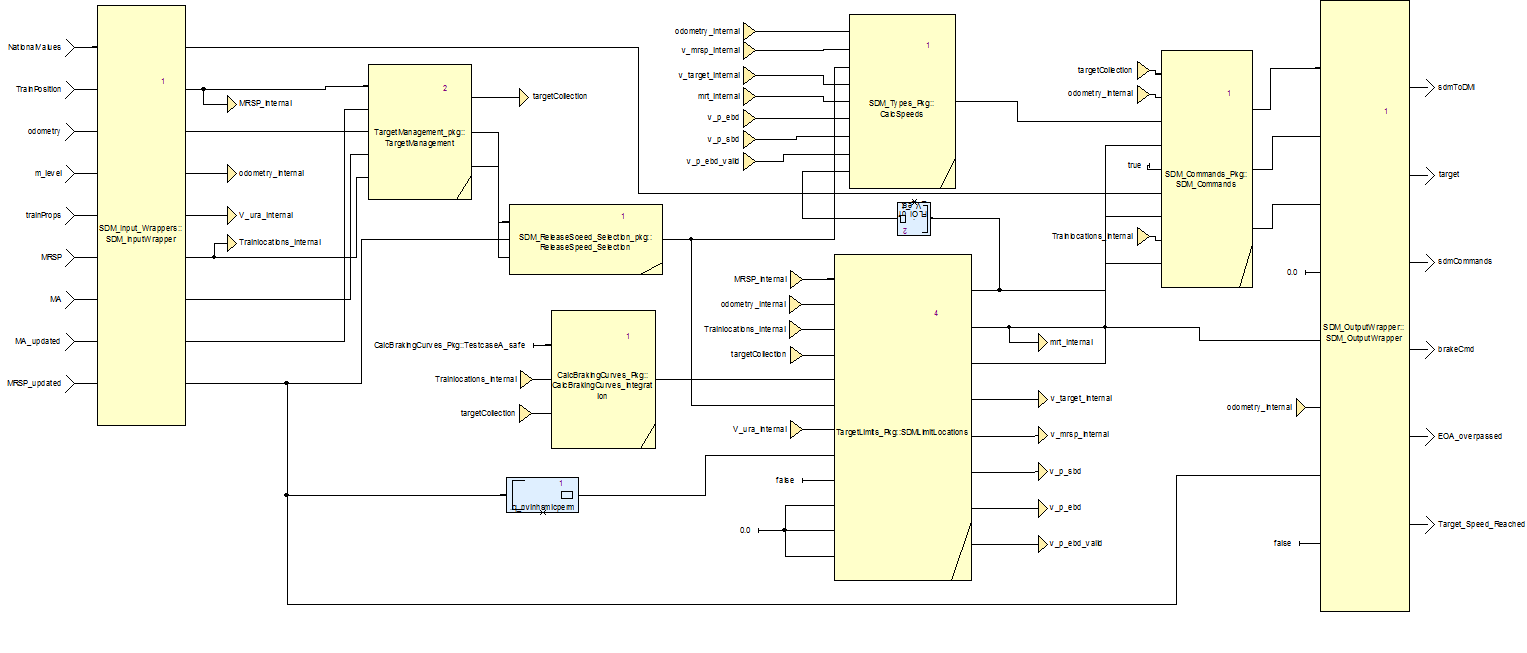
\includegraphics[width=0.95\textheight, angle=90]{../images/speedsupervision.png}
\caption{Structure of component SpeedSupervision\_Integration.}\label{f:ssv}
\end{figure}



\subsubsection{Inputs}\label{s:SDM_inputs}

\paragraph{National Values}

\begin{longtable}{p{.25\textwidth}p{.7\textwidth}}
\toprule
Input name				& NationalValues \\
\midrule
Description				& This input is packet 3 or 203 of \cite[Chapt.~8]{subset-026}, describing the national values.  \\
\midrule
Source					& TrackAtlas; current release, hard wired constant: cP3NationalValuesUtrechtAmsterdam \\
\midrule
Type					& P3\_NationalValues\_T \\
\midrule
Valid range of values	& P3\_NationalValues\_T is a complex data type, valid ranges are specified in SRS Subset-026-7, no further checks are done here. \\
\midrule
Behaviour when value is at boundary	& n/a \\
\midrule
Behaviour for values out of valid range	& n/a \\
\midrule
Behaviour when value is erroneous, absent or unwanted (i.e. spurious) & Not checked; node must not be called without reasonable National Value. \\
\bottomrule
\end{longtable}


\paragraph{Train Position}

\begin{longtable}{p{.25\textwidth}p{.7\textwidth}}
\toprule
Input name				& TrainPosition \\
\midrule
Description				& This input is the current train position. \\
\midrule
Source					& calculateTrainPosition \\
\midrule
Type					& trainPosition\_T \\
\midrule
Valid range of values	& trainPosition\_T is a complex data type. Value valid must not be false for proper function and it may not be properly checked in current release. Furthermore, reversing (decreasing positions, reverse flag set) is currently NOT supported and leads to undefined behaviour. No brake will be thrown in this occasion.
\todo[inline]{To be completed}\\
\midrule
Behaviour when value is at boundary	& Not checked, may overflow. \\
\midrule
Behaviour for values out of valid range	& Currently not checked. \\
\midrule
Behaviour when value is erroneous, absent or unwanted (i.e. spurious) & Not checked; node must not be called without reasonable position data. Valid flag is not checked (bug), as SDM has not yet implemented exception handling on inacceptable input data. \\
\bottomrule
\end{longtable}


\paragraph{Odometry}

\begin{longtable}{p{.25\textwidth}p{.7\textwidth}}
\toprule
Input name				& odometry \\
\midrule
Description				& This input is the odometry data. \\
\midrule
Source					& API\_Odometry \\ 
\midrule
Type					& odometry\_T \\
\midrule
Valid range of values	& complex data type \\
 & used fields are: \\
 & - acceleration: Obu\_BasicTypes\_Pkg::A\_internal\_Type. No valid range defined, neither checked. \\
 & - motionState: [noMotion | Motion] (enum type) \\
 & - motionDirection: is NOT evaluated currently which leads to erroneous behaviour when driving anti-nominal direction.\\
\midrule
Behaviour when value is at boundary	& Possible overflow not evaluated. \\
\midrule
Behaviour for values out of valid range	& Not checked. \\
\midrule
Behaviour when value is erroneous, absent or unwanted (i.e. spurious) & Not handled, valid data is expected for valid function. Valid flag is not checked (bug), as SDM has not yet implemented exception handling on inacceptable input data.\\
\bottomrule
\end{longtable}


\paragraph{Train Properties}

\begin{longtable}{p{.25\textwidth}p{.7\textwidth}}
\toprule
Input name				& trainProps \\
\midrule
Description				& This input is a set of train related properties. \\
\midrule
Source					& maintainTrainProperties \\ 
\midrule
Type					& trainProperties\_T \\
\midrule
Valid range of values	& trainProperties\_T is a complex type but referenced only d\_baliseAntenna\_2\_frontend.nominal: Obu\_BasicTypes\_Pkg::L\_internal\_Type No valid range defined, neither checked. \\
\midrule
Behaviour when value is at boundary	& n/a \\
\midrule
Behaviour for values out of valid range	& n/a \\
\midrule
Behaviour when value is erroneous, absent or unwanted (i.e. spurious) & Value is only evaluated in Level 1. Low values (e.g. invalid-default 0) will lead to early trip, brake and alike. Larger values will lead to late braking, possibly numeric overflow. \\
\bottomrule
\end{longtable}


\paragraph{Train Data}

\begin{longtable}{p{.25\textwidth}p{.7\textwidth}}
\toprule
Input name				& trainData \\
\midrule
Description				& This input is a set of train related inputs from the TIU. \\
\midrule
Source					& manageTrainData \\ 
\midrule
Type					& trainData\_T \\
\midrule
Valid range of values	& trainData\_T is a complex type. No valid range defined, neither checked. The source is trusted. \\
\midrule
Behaviour when value is at boundary	& n/a \\
\midrule
Behaviour for values out of valid range	& n/a \\
\midrule
Behaviour when value is erroneous, absent or unwanted (i.e. spurious) & Must be valid for SDM to function. Valid flag is not checked (bug), as SDM has not yet implemented exception handling on inacceptable input data. \\
\bottomrule
\end{longtable}

\paragraph{Track Data}

\begin{longtable}{p{.25\textwidth}p{.7\textwidth}}
\toprule
Input name				& dataFromTrackAtlas \\
\midrule
Description				& This input is a set of track related input data, containing the MRSP, the Gradient Profile and the Movement Authority. And its associated update flags to opimize data handling.\\
\midrule
Source					& TrackAtlas \\ 
\midrule
Type					& DataForSupervision\_nextGen\_t \\
\midrule
Valid range of values	& DataForSupervision\_nextGen\_t is a wrapper the three mentioned complex types. The fresh-flags are seen as an optimization hint. From specification, all three containers must contain valid data for SDM to function. Ranges or sanity are not checked. The source is trusted.
\begin{description}
\item[MA] Must always contain a valid Movement Authority, else the brake is commanded.
\item[GradientProfile] As per SRS, this must always contain a valid description up to the end of the MA.
\item[MRSP] Must at least a profile for the train's maximum speed, if no other restriction is known.
\end{description}\\
\midrule
Behaviour when value is at boundary	& n/a \\
\midrule
Behaviour for values out of valid range	& If the MA is not valid the brake should be commanded. \\
\midrule
Behaviour when value is erroneous, absent or unwanted (i.e. spurious) & Absence of minimal MRSP is not detected but trusted. Validity of MA is not checked up front.\\
\bottomrule
\end{longtable}


\subsubsection{Outputs}\label{s:SDM_outputs}

\paragraph{sdmToDMI}

\begin{longtable}{p{.25\textwidth}p{.7\textwidth}}
\toprule
Output name				& sdmToDMI \\
\midrule
Description				& This output contains information about different speeds and positions and the current supervision status. This information shall be displayed to the driver. \\
\midrule
Destination				& 
\begin{itemize}
\item TrackAtlas (\ref{s:manage_track_data_inputs})
\item manageDMI\_output (\ref{f:ManageDMIOutput})
\item ROOT\_integration 
\end{itemize} \\
\midrule
Type					& speedSupervisionForDMI\_T (complex)\\
\midrule
Valid range of values	& speedSupervisionForDMI\_T is a complex data type. Values are given for each element. Format is: Type Name: range/list of value.
\begin{itemize}
\item bool valid: [true, false] true, if internal state of speed monitoring is defined [CSM, TSM, RSM]; false, if it is undefined
\item V\_internal\_Type targetSpeed, permittedSpeed, releaseSpeed, interventionSpeed: 0 or above, not internally limited; set to cDMIUnknownSpeed (-1) if not defined
\item L\_internal\_Type location\_brake\_curve\_starting\_point, locationBrakeTarget, distanceIndicationPoint: calculated locations
\item M\_SupervisionDisplay\_T supervisionDisplay: [supDis\_normal, supDis\_indication, supDis\_overspeed, supDis\_warning, supDis\_intervention]
\item M\_SUPERVISION\_STATUS sup\_status: [CSM, TSM, RSM, unknown], PIM is not referenced
\end{itemize}\\
\midrule
Behaviour when value is at boundary	& n/a \\
\midrule
Behaviour for values out of valid range	& Location values may not be meaningful in some situations. This is not directly linked to the specific items but maybe accessible from further context such as supervisionDisplay and sup\_status.  \\
\midrule
Behaviour when value is erroneous, absent or unwanted (i.e. spurious) & Valid can be false in case of initialization. All values must be disregarded then. \\
\bottomrule
\end{longtable}


\paragraph{target}\label{p:SDM_target}

\begin{longtable}{p{.25\textwidth}p{.7\textwidth}}
\toprule
Output name				& target \\
\midrule
Description				& This output is the most restrictive displayed target (MRDT). \\
\midrule
Destination				& n/a, null-sink \\ 
\midrule
Type					& Target\_T (complex)\\
\midrule
Valid range of values	& Target\_T is a complex data type. Values are given for each element. Format is: Type Name: range/list of value.
\begin{itemize}
\item bool valid: [true, false] true, if targetType is other than invalid
\item V\_internal\_Type speed: permitted speed from target location
\item L\_internal\_Type distance: location of brake target
\item TargetType\_T targetType:
\begin{description}
\item[EoA] End of Authority (speed must be = 0)
\item[SvL] Supervised Location (speed must be = 0)
\item[MRSP] Speed Profile, Speed restriction (speed > 0)
\item[LoA] Limit of Authority (speed > 0)
\item[invalid] currently no brake target known (e.g. after trip)
\end{description}
\end{itemize}\\
\midrule
Behaviour when value is at boundary	& n/a \\
\midrule
Behaviour for values out of valid range	& Valid target values of speed and distance are not artificially limited to a sane range and are passed through data from track input.\\
\midrule
Behaviour when value is erroneous, absent or unwanted (i.e. spurious) & .valid may be false if no target is supervised or known, other values of this output must be ignored then. \\
\bottomrule
\end{longtable}


\paragraph{sdmCommands}

\begin{longtable}{p{.25\textwidth}p{.7\textwidth}}
\toprule
Output name				& sdmCommands \\
\midrule
Description				& This output gives some intermediate results of operator SDM\_Commands. It is currently used for test purposes only. \\
\midrule
Destination				& n/a, null-sink \\ 
\midrule
Type					& SDM\_Commands\_T (complex) \\
\midrule
Valid range of values	& Containing values are either boolean command-trigger flags, the internal state of the SDM\_commands state-machine or speed/distance types with guarding bool valid flag. For in-depth description see generated documentation.\\
\midrule
Behaviour when value is at boundary	& n/a \\
\midrule
Behaviour for values out of valid range	& 
\begin{itemize}
\item Bool are always in range.
\item The internal state SupervisionStatus\_T is Undefined\_Supervision at initialization and renders the output sdmToDMI's valid flag to false.
\item Speeds estimatedSpeed, permittedSpeed, releaseSpeed, mrdtSpeed, sbiSpeed and distance targetDistance must be ignored and contain invalid values if the corresponding valid-flag is false. Valid-marked outputs are not artificially limited to a sane range and rely on correctly specified algorithms.
\end{itemize}\\
\midrule
Behaviour when value is erroneous, absent or unwanted (i.e. spurious) & Overall .valid is always set, individual speeds have their corresponding valid flag. Values may not have a valid output depending on the situation. \\
\bottomrule
\end{longtable}

\paragraph{brakeCmd}

\begin{longtable}{p{.25\textwidth}p{.7\textwidth}}
\toprule
Output name				& brakeCmd \\
\midrule
Description				& This output is the brake command, indicating whether performing the service brake and/or the emergency brake have been commanded. \\
\midrule
Destination				& 
\begin{itemize}
\item TIU\_OutputIntegration (\ref{f:manageTIUOutput})
\item manageDMI\_output (\ref{f:ManageDMIOutput})
\item ROOT\_integration 
\end{itemize} \\
\midrule
Type					& Brake\_command\_T (complex)\\
\midrule
Valid range of values	& Brake\_command\_T is a complex data type. Values are given foreach element. Format is: Type Name: range/list of value
\begin{itemize}
\item bool valid: true (constant)
\item M\_brake\_signal\_command\_T m\_servicebrake\_cm:
\begin{description}
\item[brake\_signal\_command\_not\_defined] No change of brake state requested, keep last.
\item[apply\_brake] service brakes must be applied
\item[release\_brake] service brakes must be released
\end{description}
\item M\_brake\_signal\_command\_T m\_emergencybrake\_cm:
\begin{description}
\item[brake\_signal\_command\_not\_defined] No change of brake state requested, keep last.
\item[apply\_brake] emergency brakes must be applied
\item[release\_brake] emergency brakes must be released
\end{description}
\end{itemize}
Brake commands are edge triggered and may only be defined in a single cycle. \\
\midrule
Behaviour when value is at boundary	& n/a \\
\midrule
Behaviour for values out of valid range	& n/a \\
\midrule
Behaviour when value is erroneous, absent or unwanted (i.e. spurious) & brakeCmd is constantly valid, but may not contain a command change. \\
\bottomrule
\end{longtable}


\paragraph{EOA\_overpassed}

\begin{longtable}{p{.25\textwidth}p{.7\textwidth}}
\toprule
Output name				& EOA\_overpassed \\
\midrule
Description				& This output is true if the end of authority has been overpassed and false otherwise. In Level 1 this is compensated by the antenna offset.\\
\midrule
Destination				& n/a, null-sink in current release \\ 
\midrule
Type					& bool \\
\midrule
Valid range of values	& \begin{description}
                            \item[true] The train's front end has passed the end of authority
                            \item[false] The end of authority is ahead of the train.
                          \end{description}\\
\midrule
Behaviour when value is at boundary	& n/a \\
\midrule
Behaviour for values out of valid range	& n/a \\
\midrule
Behaviour when value is erroneous, absent or unwanted (i.e. spurious) & n/a \\
\bottomrule
\end{longtable}


\paragraph{Target\_Speed\_Reached}

\begin{longtable}{p{.25\textwidth}p{.7\textwidth}}
\toprule
Output name				& Target\_Speed\_Reached \\
\midrule
Description				& This output is true if the current speed is greater than or equal the target speed and false otherwise. \\
\midrule
Destination				& n/a, null-sink in current release \\ 
\midrule
Type					& bool \\
\midrule
Valid range of values	&
\begin{description}
\item[true] The current speed is greater than or equal to the target speed or target is invalid
\item[false] The current speed is less than the target speed
\end{description}
Value must be ignored, if output target (\ref{p:SDM_target}) is invalid.\\
\midrule
Behaviour when value is at boundary	& n/a \\
\midrule
Behaviour for values out of valid range	& n/a \\
\midrule
Behaviour when value is erroneous, absent or unwanted (i.e. spurious) & n/a \\
\bottomrule
\end{longtable}


\subsection{Subcomponents}\label{s:SDM_subcomponents}

\subsubsection{SDM\_InputWrapper}
%set the master document for easy compilation
%!TEX root = ../D3_5_3.tex

\paragraph{Component Requirements}

\begin{longtable}{p{.25\textwidth}p{.7\textwidth}}
\toprule
Component name			& SDM\_InputWrapper \\
\midrule
Link to SCADE model		& {\footnotesize \url{https://github.com/openETCS/modeling/tree/master/model/Scade/System/ObuFunctions/SpeedSupervison/SpeedSupervision_Integration}} \\
\midrule
SCADE designer			& Benjamin Beichler, University of Rostock\newline
Thorsten Schulz, University of Rostock \\
\midrule
Description				& The motivation for this operator is to convert all inputs of SDM that contain information about length, speed, distance, and acceleration defined as integer into \texttt{real} to allow automatically the highest precision in the calculations by the meaning of floating point operations. In addition, to ease the modeling, inside block ``Speed Supervision'' only units meters ($[m]$), seconds($[s]$), meters per second($[\frac{m}{s}]$), and meters per square second($[\frac{m}{s^{2}}]$) are used.

This operator forwards input messages, takes data from complex data types or transforms inputs messages into an internal type thereby converting int to real. \\
\midrule
Input documents	& 
Subset-026, Chapter 3.13, (not specific, helper function)\\
\midrule
Safety integrity level		& 4 \\
\midrule
Time constraints		& n/a \\
\midrule
API requirements 		& n/a \\
\bottomrule
\end{longtable}


\paragraph{Interface}

For an overview of the interface of this internal component we refer to the SCADE model (cf.~link above) respectively the SCADE generated documentation.

\subsubsection{TargetManagement}
%set the master document for easy compilation
%!TEX root = ../D3_5_2.tex

\paragraph{Component Requirements}

\begin{longtable}{p{.25\textwidth}p{.7\textwidth}}
\toprule
Component name			& TargetManagement \\
\midrule
Link to SCADE model		& {\footnotesize \url{???}} \\
\midrule
SCADE designer			& Christian Stahl, TWT \\
\midrule
Description				&This operator calculates/updates the list of targets to be supervised by the block ``Train Supervision''. Taking the current movement authority, the most restrictive speed profile and the current maximum safe front end position as an input, the operator outputs a single End of Authority target, a list of all MRSP-Targets and a list of all LoA-Targets.

\subparagraph*{Derivation of Targets from Movement Authority Sections}
The sections of the \emph{Movement Authority} could cause two types of targets:
\begin{description}
\item[End Of Authority(EoA)] only one could exist and this is only in the \emph{end section} of the \emph{MA}
\item[Limit of Authority (LoA)] is possibly in every section of the \emph{MA} except the end section
\end{description}
In every cycle in which the MA is updated, the operator iterates through the entire MA and puts all speed limitations by \emph{LoA}s into a list of targets. The end section is used to derived the \emph{EoA} target. All LoA targets are sorted by location.

\subparagraph*{Derivation of Targets from MRSP}
According to \cite[Chapt.~3.13.8.2]{subset-026}, every speed decrease of the MRSP is used to derive a target. Therefore in every cycle in which the MRSP is updated, the operator iterates through the entire MRSP searching for all MRSP targets. For this purpose, every element of the MRSP is compared with its successor.

\subparagraph*{Update of Targets}
In every cycle the operator monitors whether all targets are already passed. To this end, it iterates over the list of targets comparing the current max safe front end position with the target position. \\
\midrule
Input documents	& 
Subset-026, Chapter 3.13.8.2: Determination of the supervised targets \\
\midrule
Safety integrity level		& 4 \\
\midrule
Time constraints		& [If applicable description of time constraints, otherwise n/a] \\
\midrule
API requirements 		& [If applicable description of API requirements, otherwise n/a] \\
\bottomrule
\end{longtable}

\subsubsection{AGradient}
%set the master document for easy compilation
%!TEX root = ../D3_5_3.tex

\paragraph{Component Requirements}

\begin{longtable}{p{.25\textwidth}p{.7\textwidth}}
\toprule
Component name			& AGradient \\
\midrule

Link to SCADE model		& {\footnotesize \url{https://github.com/openETCS/modeling/tree/master/model/Scade/System/ObuFunctions/SpeedSupervisonSDM_GradientAcceleration}} \\
\midrule
SCADE designer			& Benjamin Beichler, University of Rostock\\
\midrule
Description				& This operator translates the incoming gradient profile from track data to acceleration values under consideration of train length compensation.\\
\midrule
Input documents	& 
Subset-026, Chapter 3.13.4: Acceleration / Deceleration due to gradient \\
\midrule
Safety integrity level	& 4 \\
\midrule
Time constraints		& n/a \\
\midrule
API requirements 		& n/a \\
\bottomrule
\end{longtable}


\paragraph{Interface}

For an overview of the interface of this internal component we refer to the SCADE model (cf.~link above) respectively the SCADE generated documentation.

\subsubsection{ABrakeFactory}
%set the master document for easy compilation
%!TEX root = ../D3_5_3.tex

\paragraph{Component Requirements}

\begin{longtable}{p{.25\textwidth}p{.7\textwidth}}
\toprule
Component name			& ABrakeFactory \\
\midrule

Link to SCADE model		& {\footnotesize \url{https://github.com/openETCS/modeling/tree/master/model/Scade/System/ObuFunctions/SpeedSupervison/SDM_Models}} \\
\midrule
SCADE designer			& Thorsten Schulz, University of Rostock\\
\midrule
Description				& This operator implements the braking models. At this stage only the lamda trains (conversion) model is implemented. The output of the conversion model are a location independent, but highly National Values dependent, braking curves. One for the service brake and one for the emergency brake. As a side product, the model related brake build-up times are also generated.\\
\midrule
Input documents	& 
Subset-026, Chapter 3.13.2.2.3 Braking Models, Chapter 3.13.2.2.4,5 Brake Position, Percentage, Chapter 3.13.2.3.7 National Values for SDM, Chapter 3.13.3 Conversion Models, 3.13.6 Calculation of the deceleration and brake build-up times \\
\midrule
Safety integrity level		& 4 \\
\midrule
Time constraints		& n/a \\
\midrule
API requirements 		& n/a \\
\bottomrule
\end{longtable}


\paragraph{Interface}

For an overview of the interface of this internal component we refer to the SCADE model (cf.~link above) respectively the SCADE generated documentation.

\subsubsection{addGradient}
%set the master document for easy compilation
%!TEX root = ../D3_5_3.tex

\paragraph{Component Requirements}

\begin{longtable}{p{.25\textwidth}p{.7\textwidth}}
\toprule
Component name			& addGradient \\
\midrule

Link to SCADE model		& {\footnotesize \url{https://github.com/openETCS/modeling/tree/master/model/Scade/System/ObuFunctions/SpeedSupervison/SDM_Models}} \\
\midrule
SCADE designer			& Thorsten Schulz, University of Rostock\\
\midrule
Description				& This operator is part of SDM\_Models and is merging the gradient acceleration into the curve brake model curve, producing a location dependent braking curve. It twice, for the emergency curve and the service braking curve resepctively\\
\midrule
Input documents	& 
Subset-026, Chapter 3.13.6.2.1.3 and 3.13.6.4.3 Calculation of the deceleration and brake build-up times \\
\midrule
Safety integrity level		& 4 \\
\midrule
Time constraints		& n/a \\
\midrule
API requirements 		& n/a \\
\bottomrule
\end{longtable}


\paragraph{Interface}

For an overview of the interface of this internal component we refer to the SCADE model (cf.~link above) respectively the SCADE generated documentation.

\subsubsection{CalcBrakingCurves\_Integration}
%set the master document for easy compilation
%!TEX root = ../D3_5_3.tex

\paragraph{Component Requirements}

\begin{longtable}{p{.25\textwidth}p{.7\textwidth}}
\toprule
Component name			& CalcBrakingCurves\_Integration \\
\midrule
Link to SCADE model		& {\footnotesize \url{https://github.com/openETCS/modeling/tree/master/model/Scade/System/ObuFunctions/SpeedSupervison/CalcBrakingCurves}} \\
\midrule
SCADE designer			& Benjamin Beichler, University of Rostock \\
\midrule
Description				& For each type of target a certain braking curve has to be calculated. This curve enables proactive monitoring of the train's speed. A reverse lookup on this braking curve indicates, where the train has to start braking given the current speed. The braking curve does not depend on the actual train status. As a consequence the braking curve stays constant over time. As a legitimate simplification the calculation of the braking curve is not extended past the estimated front end position of the train. \\
\midrule
Input documents	& 
Subset-026, Chapter 3.13.8.3: Emergency Brake Deceleration curves (EBD)\newline
Subset-026, Chapter 3.13.8.4: Service Brake Deceleration curves (SBD)\newline
Subset-026, Chapter 3.13.8.5: Guidance curves (GUI) \\
\midrule
Safety integrity level		& 4 \\
\midrule
Time constraints		& n/a \\
\midrule
API requirements 		& n/a \\
\bottomrule
\end{longtable}


\paragraph{Interface}

For an overview of the interface of this internal component we refer to the SCADE model (cf.~link above) respectively the SCADE generated documentation.

\subsubsection{SDMLimitLocations}
%set the master document for easy compilation
%!TEX root = ../D3_5_2.tex

\paragraph{Component Requirements}

\begin{longtable}{p{.25\textwidth}p{.7\textwidth}}
\toprule
Component name			& SDMLimitLocations \\
\midrule
Link to SCADE model		& {\footnotesize \url{???}} \\
\midrule
SCADE designer			& ??? \\
\midrule
Description				& This operator calculates the various locations needed to determine the speed and distance monitoring commands. The current implementation of functionality is stateless and requires a complete recalculation each cycle. 

This operator gathers all necessary input values and computes some frequently used intermediate values in the operators \texttt{surplusTractionDeltas} and \texttt{$v_{\mathit{bec}}$}. The other input preparation operator is the \texttt{TargetSelector} whose main task is to dissect the list of targets to find the Most Restrictive Target. The accompanying braking curves are extracted and promoted to trailing location calculations. Also the special values of the EOA are exposed.

The operator creates the requested values for the commands package. These are in particular the preindication locations for EBD and SBD based targets, the release speed monitoring start locations, the locations for target speed monitoring of the I-, W-, P- and FLOI-curve, the related FLOI speed and the location of the permitted speed supervision limit. Included in the output are also certain flags for the validity of linked values.\\
\midrule
Input documents	& 
Subset-026, Chapter 3.13.9: Supervision Limits \newline
Subset-026, Chapter 5.3.1.2: $f_{41}$ -- accuracy of speed known on-board\newline
Subset-026, Chapter 3.13.10: Monitoring Commands as reference for required outputs of this module \\
\midrule
Safety integrity level		& 4 \\
\midrule
Time constraints		& [If applicable description of time constraints, otherwise n/a] \\
\midrule
API requirements 		& [If applicable description of API requirements, otherwise n/a] \\
\bottomrule
\end{longtable}

%\subsubsection{CalcSpeeds}
%%set the master document for easy compilation
%!TEX root = ../D3_5_3.tex

\paragraph{Component Requirements}

\begin{longtable}{p{.25\textwidth}p{.7\textwidth}}
\toprule
Component name			& CalcSpeeds \\
\midrule
Link to SCADE model		& {\footnotesize \url{https://github.com/openETCS/modeling/tree/master/model/Scade/System/ObuFunctions/SpeedSupervison/SpeedSupervision\_Integration}} \\
\midrule
SCADE designer			& Benjamin Beichler, University of Rostock \\
\midrule
Description				& This operator calculates some speeds needed to determine the speed and distance monitoring commands. This operator will be integrated into other operators in the next iteration.\\
\midrule
Input documents	& 
Subset-026, Chapter 3.8: Movement authority \\
\midrule
Safety integrity level		& 4 \\
\midrule
Time constraints		& n/a \\
\midrule
API requirements 		& n/a \\
\bottomrule
\end{longtable}


\paragraph{Interface}

For an overview of the interface of this internal component we refer to the SCADE model (cf.~link above) respectively the SCADE generated documentation.
%
%\subsubsection{ReleaseSpeed\_Selection}
%%set the master document for easy compilation
%!TEX root = ../D3_5_2.tex

\paragraph{Component Requirements}

\begin{longtable}{p{.25\textwidth}p{.7\textwidth}}
\toprule
Component name			& ReleaseSpeed\_Selection \\
\midrule
Link to SCADE model		& {\footnotesize \url{???}} \\
\midrule
SCADE designer			& ??? \\
\midrule
Description				&This operator outputs the release speed which can be given either by the national values or the movement authority. This operator will be integrated into other operators in the next iteration.\\
\midrule
Input documents	& 
Subset-026, Chapter 3.8: Movement authority \\
\midrule
Safety integrity level		& 4 \\
\midrule
Time constraints		& [If applicable description of time constraints, otherwise n/a] \\
\midrule
API requirements 		& [If applicable description of API requirements, otherwise n/a] \\
\bottomrule
\end{longtable}


\paragraph{Interface}

For an overview of the interface of this internal component we refer to the SCADE model (c.f.~link above) respectively the SCADE generated documentation.
%
\subsubsection{SDM\_Commands}
%set the master document for easy compilation
%!TEX root = ../D3_5_3.tex

\paragraph{Component Requirements}

\begin{longtable}{p{.25\textwidth}p{.7\textwidth}}
\toprule
Component name			& SDM\_Commands \\
\midrule
Link to SCADE model		& {\footnotesize \url{https://github.com/openETCS/modeling/tree/master/model/Scade/System/ObuFunctions/SpeedSupervison/SDM_Commands}} \\
\midrule
SCADE designer			& Christian Stahl, TWT; (cur. maintainer Thorsten Schulz, University of Rostock) \\
\midrule
Description				& This operator models the speed and distance monitoring commands. More precisely, it triggers the service or emergency brake and outputs the current supervision status of the OBU together with information on speeds and locations to the driver.

The OBU can be in any of three types of speed and distance monitoring modes: ceiling speed monitoring, release speed monitoring and target speed monitoring. We use a state machine to model the switching between the three modes: each state models a mode and a transition between to states is enabled if the condition two switch between the two corresponding modes is evaluated to true. In each mode, the OBU can be in up to five different supervision stati. The behavior of changing from one status to another is also modeled as a state machine. As a result, the model is a hierarchical state machine.\\
\midrule
Input documents	& 
Subset-026, Chapter 3.13.10: Speed and distance monitoring commands \\
\midrule
Safety integrity level		& 4 \\
\midrule
Time constraints		& n/a \\
\midrule
API requirements 		& n/a \\
\bottomrule
\end{longtable}


\paragraph{Interface}

For an overview of the interface of this internal component we refer to the SCADE model (c.f.~link above) respectively the SCADE generated documentation.

%\subsubsection{SDM\_OutputWrapper}
%%set the master document for easy compilation
%!TEX root = ../D3_5_3.tex

\paragraph{Component Requirements}

\begin{longtable}{p{.25\textwidth}p{.7\textwidth}}
\toprule
Component name			& SDM\_OutputWrapper \\
\midrule
Link to SCADE model		& {\footnotesize \url{https://github.com/openETCS/modeling/tree/master/model/Scade/System/ObuFunctions/SpeedSupervison/SpeedSupervision_Integration}} \\
\midrule
SCADE designer			& Benjamin Beichler,University of Rostock\newline
Thorsten Schulz, University of Rostock \\
\midrule
Description				& This operator is the counterpart to operator SDM\_OutputWrapper---that is, it converts all internal outputs of SDM that contain information about length, speed, distance, and acceleration defined as real into int, such that all other blocks can stick to their types and also performs the calculation into units used by the environment.

This operator forwards input messages and transforms inputs messages into an internal type thereby converting real to int.\\
\midrule
Input documents	& 
Subset-026, Chapter 3.13.10: Speed and distance monitoring commands\\
\midrule
Safety integrity level		& 4 \\
\midrule
Time constraints		& n/a \\
\midrule
API requirements 		& n/a \\
\bottomrule
\end{longtable}



\paragraph{Interface}

For an overview of the interface of this internal component we refer to the SCADE model (c.f.~link above) respectively the SCADE generated documentation.

%